\chapter{同调}
\label{chap:homology}

用三根铁丝焊成一个三角形框，再剪一块三角形纸片把框填满。两件东西有相同的三个顶点和三条边，只记录“哪两点直接相连”的图分不出它们。可是框的中间有一个洞，纸片没有。

圆周与环带的关系正好相反。环带比圆周“厚”，两者不同胚；但环带可以沿半径连续地压扁到中间的圆周上，洞始终还在。本章研究怎样用可以计算的代数量辨认这样的洞，以及这些量在哪些连续变形下保持不变。

全章分四步。第~\ref{sec:homol-homotopy}节用同伦描述允许的连续变形，用同伦等价和形变收缩说明环带为何与圆周“有同样的洞”。第~\ref{sec:homol-simplicial-complexes}节用有限单纯复形记录点、边和填充，再把这份记录实现为空间。

第~\ref{sec:homol-simplicial-homology}节在实数系数下把单纯形组合成向量，边界映射成为矩阵，“闭合”成为零空间，“已被填掉”成为列空间，洞的个数归结为矩阵的秩。第~\ref{sec:homol-singular-homology}节用标准单纯形到空间的连续映射，把同样的构造搬到任意拓扑空间上，并证明它在同伦下不变。由此算出圆周、环带、圆盘和球面的同调，也看清同调相同并不意味着同胚。

本章的拓扑语言来自第~\ref{chap:topological-spaces}章，链、核、像与商空间都回用有限维线性代数。同调在流形上的意义在第~\ref{chap:manifold-basics}章讨论，从有限点云恢复同调、跨尺度的持久同调在第~\ref{chap:manifold-recovery}章讨论。本章的例子都小到可以手算。

\section{同伦}
\label{sec:homol-homotopy}

同胚要求两个空间的点一一对应，并且对应在两个方向上都连续。这个要求很严，常常把我们心目中“形状相同”的空间分开。下面比较平面中的单位圆周和环带，二者都取欧氏空间的子空间拓扑：
\[
 S^1=\{\bm x\in\mathbb R^2:\lVert\bm x\rVert_2=1\},\qquad
 A=\{\bm x\in\mathbb R^2:1\leq\lVert\bm x\rVert_2\leq2\}.
\]

两者都围着同一个洞，但它们不同胚。区分的办法是看去掉两个点之后还剩下什么。图~\ref{fig:homol-remove-two-points}画出了这两种情形。

\begin{BookInlineFigure}
  \centering
  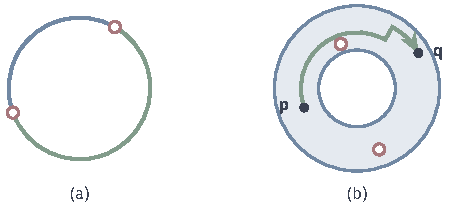
\includegraphics[width=76.962mm]{figures/04-spaces-measures-and-geometry/01-topology-and-metric/tikz/homol-remove-two-points/figure.pdf}
  \caption{圆周与环带各去掉两个点（红色空心点）。(a)圆周断成蓝、绿两段互不相连的开弧。(b)环带中任意两点$\bm p,\bm q$仍可相连：绿色路径先沿圆弧绕到一条避开去掉点的射线，沿射线移动，再沿另一段圆弧到达$\bm q$。}
  \label{fig:homol-remove-two-points}
\end{BookInlineFigure}

从$S^1$中去掉两个不同的点，剩下两段互不相交的开弧，空间不连通。从$A$中去掉任意两点，剩下的部分却仍然路径连通，理由如下。

任取剩下的两点$\bm p,\bm q$。去掉的两点只占两个半径值，所以可以在$\lVert\bm p\rVert_2$附近取一个半径$r_p\in[1,2]$，使半径为$r_p$的圆避开去掉的点，并且从$\bm p$沿半径走到这个圆的短线段也避开它们。对$\bm q$同样取$r_q$。

去掉的点只占两个方向，所以还可以取一条不经过它们的射线。于是从$\bm p$出发沿短线段到半径为$r_p$的圆，沿圆走到射线上，沿射线走到半径为$r_q$的圆，沿这个圆走到$\bm q$的半径方向，最后沿短线段到达$\bm q$。各段首尾相接，就得到一条连接$\bm p,\bm q$的路径。

同胚把“去掉两点”对应为“去掉两点”，并且保持连通性（第~\ref{chap:topological-spaces}章）。两种结果不同，所以$S^1$与$A$不同胚。

可是环带能沿半径连续地压到圆周上，压缩中洞始终存在。要表达“有同样的洞”，需要一种比同胚宽松的比较：不再要求点一一对应，只要求能用连续变形相互转化。下面先定义映射之间的连续变形，再说明怎样把空间连续收回它的子空间。

\subsection{同伦等价}
\label{sec:homol-homotopy-equivalence}

把环带压到圆周上，可以想成一段动画：时间$t$从$0$走到$1$，$t=0$时每个点都在原处，$t=1$时每个点都落到圆周上，中间每一帧都是一个映射。动画要“不跳帧”，不能只要求每一帧连续，还要求同一个点的位置随时间连续变动。

把时间当作一个额外的坐标，这两种连续性就合成了一个条件：动画是定义在“空间$\times$时间”上的一个连续映射。

\begin{definition}[同伦]
\label{def:homol-homotopy}
设$X,Y$为拓扑空间，$f,g:X\to Y$连续，$X\times[0,1]$取乘积拓扑。若存在连续映射$H:X\times[0,1]\to Y$，使得
\begin{equation}
 H(x,0)=f(x),\qquad H(x,1)=g(x),\qquad x\in X,
 \label{eq:homol-homotopy}
\end{equation}
则称$f$与$g$\term{同伦}（homotopy），记为$f\simeq g$，称$H$为从$f$到$g$的一个同伦。
\end{definition}

记$h_t=H(\cdot,t)$，这是动画在时刻$t$的一帧。从图~\ref{fig:homol-homotopy-family}可以同时读出同伦的两种看法：横着看，$X\times[0,1]$的每条水平线给出一个映射$h_t$；竖着看，每条竖线给出一个点$x$的运动轨迹$t\mapsto h_t(x)$。

\begin{BookInlineFigure}
  \centering
  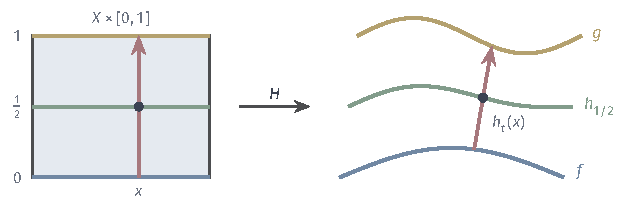
\includegraphics[width=105.971mm]{figures/04-spaces-measures-and-geometry/01-topology-and-metric/tikz/homol-homotopy-family/figure.pdf}
  \caption{同伦把矩形$X\times[0,1]$映到$Y$（此处$X$为线段，$Y$为平面）。蓝、绿、黄三条水平线分别对应$f$、$h_{1/2}$与$g$；红色竖线是固定$x$时的轨迹，它被$H$送成从$f(x)$到$g(x)$的一条路径。}
  \label{fig:homol-homotopy-family}
\end{BookInlineFigure}

$H$在乘积空间上整体连续，比每个$h_t$连续更强。例如令$h_0$为$\mathbb R$上的恒等映射，$t>0$时$h_t$恒取$0$，则每一帧都连续，点$x\neq0$却在$t=0$的瞬间跳到$0$。这样的“跳帧”被整体连续的要求排除了。

最常用的同伦是直线同伦。若$Y\subseteq\mathbb R^n$是凸集，$f,g:X\to Y$连续，令
\begin{equation}
 H(x,t)=(1-t)f(x)+tg(x).
 \label{eq:homol-straight-line-homotopy}
\end{equation}
凸性保证线段上的点仍在$Y$中；$H$由连续函数经乘法与加法得到，因而连续。所以进入凸集的任意两个连续映射都同伦，特别地，进入凸集的映射都同伦于常值映射。

\paragraph{同伦关系的性质}
后面要把同伦的映射看作“同一类”，因此先确认同伦是等价关系，并且与复合相容。

\begin{lemma}[同伦是等价关系]
\label{lem:homol-homotopy-equivalence-relation}
对固定的$X,Y$，连续映射$X\to Y$之间的同伦关系是等价关系。若$f\simeq f':X\to Y$，$g\simeq g':Y\to Z$，则$g\circ f\simeq g'\circ f'$。
\end{lemma}

\begin{proof}
自反性取同伦$H(x,t)=f(x)$，即动画一直停在第一帧。对称性把时间倒过来，若$H$从$f$到$g$，则$H(x,1-t)$从$g$到$f$。

对传递性，设$H$从$f$到$g$，$G$从$g$到$h$。把两段动画接起来，每段用一半时间播放：
\[
 K(x,t)=\begin{cases}H(x,2t),&0\leq t\leq1/2,\\ G(x,2t-1),&1/2\leq t\leq1.\end{cases}
\]
两段在$t=1/2$处都等于$g(x)$，所以$K$有定义。

$K$的连续性用闭集判断。$X\times[0,1/2]$与$X\times[1/2,1]$都是闭集，$K$在其上的限制都连续。对$Y$中任一闭集$F$，$K^{-1}(F)$是两个限制的原像之并。每个原像在相应闭子集中是闭的，因而在整个乘积中是闭的，两个闭集之并仍是闭集，所以$K$连续。

再看与复合的相容性。设$H$从$f$到$f'$，$G$从$g$到$g'$，令
\[
 K(x,t)=G(H(x,t),t).
\]
它是连续映射$(x,t)\mapsto(H(x,t),t)$与$G$的复合，前者的两个分量都连续。代入$t=0$与$t=1$，分别得到$g\circ f$与$g'\circ f'$，所以$K$就是所求的同伦。
\end{proof}

\paragraph{同伦等价与可缩空间}
同胚要求存在互逆的连续映射：去了再回来，恰好回到原处。把“恰好回到原处”放宽为“能连续变回原处”，就得到需要的比较。

\begin{definition}[同伦等价]
\label{def:homol-homotopy-equivalent}
若连续映射$f:X\to Y$与$g:Y\to X$满足
\begin{equation}
 g\circ f\simeq\operatorname{id}_X,\qquad f\circ g\simeq\operatorname{id}_Y,
 \label{eq:homol-homotopy-equivalence}
\end{equation}
则称$f$是\term{同伦等价}（homotopy equivalence），$g$是它的同伦逆，并称$X$与$Y$同伦等价，记为$X\simeq Y$。与单点空间同伦等价的空间称为\term{可缩空间}（contractible space）。
\end{definition}

同胚是同伦等价：互逆映射的复合恰好等于恒等映射。同伦等价的复合仍是同伦等价。设$f:X\to Y$的同伦逆为$g$，$f':Y\to Z$的同伦逆为$g'$，由引理~\ref{lem:homol-homotopy-equivalence-relation}的复合相容性，
\[
 (g\circ g')\circ(f'\circ f)=g\circ(g'\circ f')\circ f
 \simeq g\circ\operatorname{id}_Y\circ f=g\circ f\simeq\operatorname{id}_X,
\]
另一侧同理。所以空间之间的同伦等价也是等价关系。

可缩性有一个更直接的判据：$X$可缩，当且仅当$\operatorname{id}_X$同伦于某个常值映射。设$X\simeq\{p\}$，映射为$f:X\to\{p\}$，同伦逆$g$把$p$送到某点$x_0$，则$g\circ f$是取值$x_0$的常值映射，它同伦于$\operatorname{id}_X$。

反过来，若$\operatorname{id}_X$同伦于取值$x_0$的常值映射，取$f:X\to\{p\}$与$g(p)=x_0$。此时$g\circ f$正是这个常值映射，而$f\circ g=\operatorname{id}_{\{p\}}$自动成立。

\begin{example}[区间与圆盘可缩]
\label{ex:homol-contractible}
闭圆盘是含原点的凸集，记为
\[
 D^2=\{\bm x\in\mathbb R^2:\lVert\bm x\rVert_2\leq1\}.
\]
取直线同伦
\[
 H(\bm x,t)=(1-t)\bm x,
\]
它从恒等映射连续变到取值为原点的常值映射，所以圆盘可缩。例如点$(1,0)$在$t=1/2$时位于$(1/2,0)$，在$t=1$时到达原点。同样的公式把$[-1,1]$收缩到原点。对一般的非空凸集，任取其中一点$\bm a$，用$H(\bm x,t)=(1-t)\bm x+t\bm a$，所以区间$[0,1]$、$\mathbb R^n$及其中任何非空凸集都可缩。
\end{example}

环带是否可缩，直观上似乎一目了然：中间的洞消不掉。但要证明不存在从$\operatorname{id}_A$到常值映射的同伦，就要排除所有可能的连续变形，一个个去试做不到。这正是同调要解决的问题，第~\ref{sec:homol-homotopy-invariance}小节将给出证明。

\paragraph{同伦等价与同胚的区别}
同伦等价比同胚宽松得多。单点与区间$[0,1]$同伦等价，却不同胚，因为两者之间连双射都没有。区间与圆盘都可缩，因而同伦等价，但它们也不同胚。

区间去掉一个内点就不连通。圆盘去掉任何一点$\bm q$却仍然路径连通：任取剩下的两点，取一点$\bm m\in D^2$，使它不在过这两点的直线上；由凸性，两条线段经过$\bm m$把这两点连起来，而除这两点外它们都不在那条直线上，碰不到$\bm q$（$\bm q$若不在这条直线上，直接取线段即可）。同胚把“去掉一点”对应为“去掉一点”，所以二者不同胚。

\begin{BookInlineTable}
  \centering
  \caption{同胚与同伦等价的比较}
  \label{tab:homol-homeo-vs-homotopy}
  \begin{tabular}{lll}
    \toprule
    & 同胚 & 同伦等价 \\
    \midrule
    需要的映射 & 互逆的$f,g$ & 复合同伦于恒等映射的$f,g$ \\
    点的对应 & 一一对应 & 可以把一片压成一点 \\
    保持的信息 & 维数、局部形状等 & 连通分支、洞的个数等 \\
    区间与单点 & 不同 & 相同 \\
    环带与圆周 & 不同 & 相同 \\
    \bottomrule
  \end{tabular}
\end{BookInlineTable}

表~\ref{tab:homol-homeo-vs-homotopy}把两种比较放在一起。同伦等价忽略了维数和点的多少，只保留连续变形下不变的整体信息。表中“保持的信息”一行里的“洞的个数”，还需要用本章后面的同调来说清楚。

\subsection{形变收缩}
\label{sec:homol-deformation-retraction}

环带压向圆周的过程有一个特点：圆周上的点始终不动，其余的点最终都落到圆周上。这样的变形把空间收回到它的一个子空间，而子空间本身不受扰动。

把这个过程拆成两件事：最后的结果是一个把空间收回子空间的映射，过程是把这个映射与恒等映射连起来的同伦。

\begin{definition}[形变收缩]
\label{def:homol-deformation-retraction}
设$Y\subseteq X$为子空间。若连续映射$r:X\to Y$满足$r(a)=a$对一切$a\in Y$成立，则称$r$为\term{回缩}（retraction）。若存在连续映射$H:X\times[0,1]\to X$，满足
\begin{align}
 H(x,0)&=x,\quad H(x,1)\in Y,&x&\in X,\label{eq:homol-deformation-end}\\
 H(a,t)&=a,&a&\in Y,\ t\in[0,1],\label{eq:homol-deformation-fixed}
\end{align}
则称$H$为从$X$到$Y$的\term{形变收缩}（deformation retraction），称$Y$为$X$的形变收缩核。
\end{definition}

两条要求分工不同。式~\eqref{eq:homol-deformation-end}说变形从恒等映射出发，终点落在$Y$中；式~\eqref{eq:homol-deformation-fixed}说$Y$上的点全程固定。两条合起来，终止映射$r=H(\cdot,1)$满足$r|_Y=\operatorname{id}_Y$，是一个回缩；而$H$本身是从$\operatorname{id}_X$到$i\circ r$的同伦，其中$i:Y\to X$是包含映射。

\begin{example}[环带收向圆周]
\label{ex:homol-annulus-retraction}
对环带$A$与圆周$S^1$，令
\begin{equation}
 H(\bm x,t)=(1-t)\bm x+t\frac{\bm x}{\lVert\bm x\rVert_2}.
 \label{eq:homol-annulus-retraction}
\end{equation}
在$A$上$\lVert\bm x\rVert_2\geq1$，分母不为零，所以$H$连续。$H(\bm x,t)$与$\bm x$同方向，长度为
\[
 \lVert H(\bm x,t)\rVert_2=(1-t)\lVert\bm x\rVert_2+t\in[1,2],
\]
所以始终留在$A$中。

$t=0$时$H$是恒等映射。$t=1$时它把每点沿半径送到圆周上，例如点$(0,2)$在$t=1/2$时位于$(0,3/2)$，在$t=1$时到达$(0,1)$。若$\lVert\bm x\rVert_2=1$，则$H(\bm x,t)=\bm x$，圆周上的点不动。因此$H$是从$A$到$S^1$的形变收缩。同一公式也把去掉原点的平面$\mathbb R^2\setminus\{\bm 0\}$形变收缩到$S^1$。
\end{example}

\begin{BookInlineFigure}
  \centering
  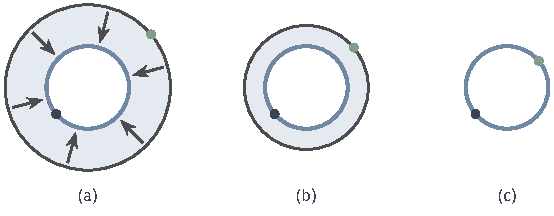
\includegraphics[width=93.832mm]{figures/04-spaces-measures-and-geometry/01-topology-and-metric/tikz/homol-annulus-retraction/figure.pdf}
  \caption{环带沿半径收向圆周，(a)(b)(c)依次是式~\eqref{eq:homol-annulus-retraction}在$t=0,\,1/2,\,1$的像。粗蓝线是单位圆周，全程不动；外缘上的绿点半径由$2$变为$3/2$，再变为$1$；圆周上的黑点始终停在原处。}
  \label{fig:homol-annulus-retraction}
\end{BookInlineFigure}

图~\ref{fig:homol-annulus-retraction}是这个过程的三帧。把它写成一般结论，形变收缩给出的正是同伦等价所需要的那对映射。

\begin{theorem}[形变收缩给出同伦等价]
\label{thm:homol-retract-equivalence}
若$Y$是$X$的形变收缩核，$r=H(\cdot,1)$为相应的回缩，$i:Y\to X$为包含映射，则$i$是同伦等价，$r$是它的同伦逆。特别地，$X\simeq Y$。
\end{theorem}

\begin{proof}
由于$r$在$Y$上是恒等映射，一侧等式严格成立：
\[
 r\circ i=\operatorname{id}_Y.
\]

另一侧，由定义，$H$满足$H(x,0)=x$与$H(x,1)=i(r(x))$，它正是从$\operatorname{id}_X$到$i\circ r$的同伦，所以$i\circ r\simeq\operatorname{id}_X$。
\end{proof}

由例~\ref{ex:homol-annulus-retraction}与定理~\ref{thm:homol-retract-equivalence}，$A\simeq S^1$。环带与圆周不同胚，却同伦等价，这正是本节开头想表达的“有同样的洞”。

\paragraph{回缩本身不够}
只有回缩而没有形变，不能得出同伦等价。取两点离散空间$X=\{0,1\}$与子空间$Y=\{0\}$，常值映射$r\equiv0$是回缩。若$i\circ r\simeq\operatorname{id}_X$，同伦限制在点$1$上就给出一条从$0$到$1$的路径，可是$X$不连通，这样的路径不存在。

所以$Y$不是$X$的形变收缩核。回缩只说“结果”：每个点都有去处。形变收缩还要求“过程”：每个点能沿连续的路径走到去处。上面的点$1$有去处，却没有路可走。

定义要求$Y$全程固定，这比同伦等价所需要的略强。若只要$X\simeq Y$，允许$Y$中的点在$Y$内部移动也够了：此时$H$限制在$Y$上给出$r\circ i\simeq\operatorname{id}_Y$，定理~\ref{thm:homol-retract-equivalence}的结论不变。保留固定条件，是因为它描述的正是“把多余部分收回、核心不动”这一具体过程；第~\ref{chap:manifold-recovery}章把点云邻域收回流形时，用的就是这种形式。

同伦等价究竟保留了什么代数信息，需要先建立同调才能回答。下一节先解决输入的问题：怎样把一个空间写成有限的数据。

\section{有限单纯复形}
\label{sec:homol-simplicial-complexes}

要计算洞，先要有能写成有限数据的空间。图是一个候选：它用顶点和边记录直接连接，也可以有环（可参考\BookChapterRef{chap:graph-objects}{卷三第1章“图与连接结构”}）。但本章开头的三角形框与三角形纸片有同一张图，三个顶点两两相邻。图中的环$0\to1\to2\to0$在框上围着一个洞，在纸片上却什么也没围住。

只记录邻接边，就丢掉了“这个环已经被填上”的信息。修补的办法是把“填充”也记下来：除了点和边，还允许记录三个顶点张成的三角形、四个顶点张成的四面体，等等。本节先建立这种有限的组合对象，再把它实现为欧氏空间中的子集，使连续映射与同伦能够作用在它上面。

\subsection{单纯复形的定义}
\label{sec:homol-complex-definition}

一个填充三角形由它的三个顶点确定，一条边由两个端点确定，所以一块“填充”可以简单地记为一个顶点子集。记录要前后一致：填入一个三角形时，它的三条边和三个顶点也必须在记录之中，否则三角形的边缘无处安放。

\begin{definition}[抽象单纯复形]
\label{def:homol-simplicial-complex}
设$V$为有限集。由$V$的非空子集组成的族$\mathcal K$称为以$V$为顶点集的\term{抽象单纯复形}（abstract simplicial complex），若
\begin{itemize}
 \item 对每个$v\in V$，$\{v\}\in\mathcal K$；
 \item 若$\sigma\in\mathcal K$且$\varnothing\neq\tau\subseteq\sigma$，则$\tau\in\mathcal K$。
\end{itemize}
$\mathcal K$中的元素称为\term{单纯形}（simplex）。含$k+1$个顶点的单纯形称为$k$维单纯形，简称$k$-单纯形；单纯形$\sigma$的非空子集称为它的\term{面}（face）。$\mathcal K$中单纯形维数的最大值称为$\mathcal K$的维数。
\end{definition}

第二条要求称为对取面封闭，它正是上面所说的“填入三角形时，边和顶点也要在”。$0$维单纯形是顶点，$1$维单纯形是边，$2$维单纯形是填充三角形，$3$维单纯形是实心四面体。

一维的单纯复形恰好就是一张简单无向图：顶点集是$V$，边集是二元单纯形的全体。单纯复形因而可以看作图向高维的推广。

记$n_k$为$\mathcal K$中$k$维单纯形的个数。若$\mathcal L\subseteq\mathcal K$本身也是单纯复形，就称$\mathcal L$为$\mathcal K$的\term{子复形}（subcomplex）。维数不超过$k$的单纯形组成的子复形称为$\mathcal K$的$k$维\term{骨架}（skeleton），记为$\mathcal K^{(k)}$；一维骨架就是$\mathcal K$的顶点与边组成的图。

\begin{example}[三角形边界与填实三角形]
\label{ex:homol-two-triangles}
取$V=\{0,1,2\}$，令
\begin{align*}
 \mathcal T_1&=\bigl\{\{0\},\{1\},\{2\},\{0,1\},\{1,2\},\{0,2\}\bigr\},\\
 \mathcal T_2&=\mathcal T_1\cup\bigl\{\{0,1,2\}\bigr\}.
\end{align*}
两者都对取面封闭。$\mathcal T_1$是一维复形，单纯形个数为$(n_0,n_1)=(3,3)$，记录三角形的边界；$\mathcal T_2$是二维复形，单纯形个数为$(n_0,n_1,n_2)=(3,3,1)$，记录填实的三角形。

它们的一维骨架相同，都是三个顶点两两相邻的图，$\mathcal T_1$是$\mathcal T_2$的子复形。集合族$\bigl\{\{0\},\{1\},\{2\},\{0,1,2\}\bigr\}$则不是单纯复形，它记录了三角形，却缺少三条边。
\end{example}

图~\ref{fig:homol-triangle-complexes}的前三幅画出了这三个集合族。比较(a)与(b)，例~\ref{ex:homol-two-triangles}说明图中的环未必对应复形中的洞：在$\mathcal T_2$中，环$0\to1\to2\to0$恰好是那个填充三角形的边界。判断一个环是否围住了洞，要看它能否被某些高维单纯形“填掉”，第~\ref{sec:homol-simplicial-homology}节用边界映射把这件事说精确。

\begin{BookInlineFigure}
  \centering
  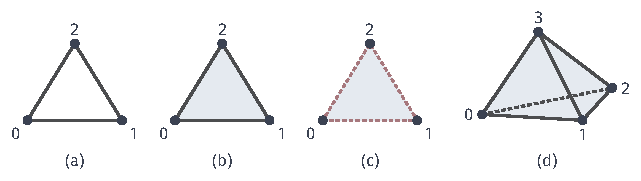
\includegraphics[width=108.532mm]{figures/04-spaces-measures-and-geometry/01-topology-and-metric/tikz/homol-triangle-complexes/figure.pdf}
  \caption{有限单纯复形及一个反例。(a)$\mathcal T_1$：三角形边界。(b)$\mathcal T_2$：填实的三角形，比(a)多一个二维单纯形（浅蓝）。(c)只有填充和顶点、没有三条边的集合族（红色虚线表示缺失的边），不对取面封闭。(d)$\mathcal S$：空心四面体表面，虚线是被遮挡的边，内部没有三维单纯形。}
  \label{fig:homol-triangle-complexes}
\end{BookInlineFigure}

\begin{example}[四面体的表面]
\label{ex:homol-tetrahedron-boundary}
取$V=\{0,1,2,3\}$，令$\mathcal S$由$V$的全部非空真子集组成，即$4$个顶点、$6$条边和$4$个三角形，单纯形个数为$(n_0,n_1,n_2)=(4,6,4)$，不含$3$维单纯形$\{0,1,2,3\}$。它记录空心四面体的表面，见图~\ref{fig:homol-triangle-complexes}(d)，中间围住一个“二维的洞”。再加上$V$本身，就得到实心四面体。
\end{example}

\subsection{几何实现}
\label{sec:homol-geometric-realization}

抽象单纯复形只是集合族，没有点、开集或连续映射。要谈论同伦，必须把它变成一个拓扑空间：每个$k$维单纯形换成一块$k$维的“实心”几何对象，再把公共的面粘在一起。

\paragraph{标准单纯形}
先定下这块几何对象。在$\mathbb R^{k+1}$中，取坐标非负且和为$1$的点，得到
\begin{equation}
 \Delta^k=\Bigl\{\bm t=(t_0,\ldots,t_k)\in\mathbb R^{k+1}:t_i\geq0,\ \sum_{i=0}^kt_i=1\Bigr\},
 \label{eq:homol-standard-simplex}
\end{equation}
称为$k$维\term{标准单纯形}（standard simplex），取$\mathbb R^{k+1}$的子空间拓扑。它是标准基向量$\bm e_0,\ldots,\bm e_k$的凸包，有界且闭，因而紧。

$\Delta^0$是一点，$\Delta^1$是线段，$\Delta^2$是三角形，$\Delta^3$是四面体，图~\ref{fig:homol-standard-simplices}画出了后三者。坐标$t_i$可以读成“$\bm e_i$的权重”：$\Delta^2$中的点$\bm t=(\frac12,\frac14,\frac14)$就是
\[
 \tfrac12\bm e_0+\tfrac14\bm e_1+\tfrac14\bm e_2,
\]
三个顶点的加权平均。把某些坐标取为零，得到的子集仍是由其余基向量张成的低维单纯形，称为$\Delta^k$的面。例如$\Delta^2$中$t_0=0$的点组成连接$\bm e_1,\bm e_2$的边。

\begin{BookInlineFigure}
  \centering
  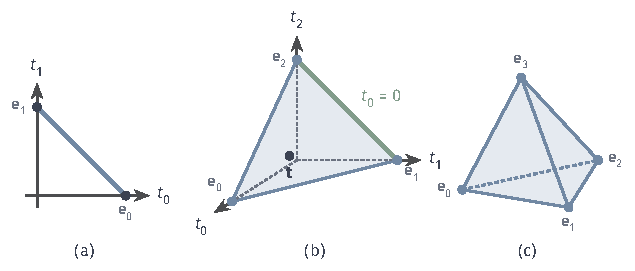
\includegraphics[width=107.453mm]{figures/04-spaces-measures-and-geometry/01-topology-and-metric/tikz/homol-standard-simplices/figure.pdf}
  \caption{标准单纯形。(a)$\Delta^1$是$\mathbb R^2$中连接$\bm e_0,\bm e_1$的线段。(b)$\Delta^2$是$\mathbb R^3$中的三角形，黑点是$\bm t=(\frac12,\frac14,\frac14)$；绿色边是$t_0=0$的面。(c)$\Delta^3$位于$\mathbb R^4$中，此处按四面体形状示意，虚线是被遮挡的边。}
  \label{fig:homol-standard-simplices}
\end{BookInlineFigure}

\paragraph{沿公共面粘合}
下面把单纯形按记录粘起来。设$\mathcal K$的顶点集为$V$。对每个单纯形$\sigma\in\mathcal K$，取一份以$\sigma$的顶点为坐标编号的几何单纯形：
\[
 \Delta^\sigma=\Bigl\{(t_v)_{v\in\sigma}:t_v\geq0,\ \sum_{v\in\sigma}t_v=1\Bigr\}.
\]

把各份放在某个欧氏空间中互不相交的位置，它们的并记为$W$，取子空间拓扑。$W$是有限个紧集之并，因而紧。若$\tau\subseteq\sigma$，则$\Delta^\tau$可以看作$\Delta^\sigma$中$\sigma\setminus\tau$各坐标为零的那个面。

在$W$上规定：$\Delta^\tau$中的点与$\Delta^\sigma$中对应面上坐标相同的点等价，并取由此生成的等价关系$\sim$。商空间$W/{\sim}$（第~\ref{chap:topological-spaces}章）就是把每个面与它在复形中对应的单纯形粘成一份，图~\ref{fig:homol-gluing}(a)(b)画的是两个三角形沿公共边粘合的情形。

\begin{BookInlineFigure}
  \centering
  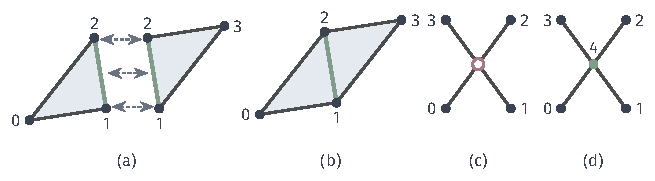
\includegraphics[width=110.973mm]{figures/04-spaces-measures-and-geometry/01-topology-and-metric/tikz/homol-gluing/figure.pdf}
  \caption{粘合与画法。(a)$\{0,1,2\}$与$\{1,2,3\}$的两份几何单纯形，公共边的两份副本为绿色，虚线箭头连接被等同的点。(b)粘合结果。(c)边$\{0,2\}$与$\{1,3\}$在纸上交叉，但红色空心点不是复形中的点。(d)加入新顶点$4$并把两条边各拆成两段之后，四条边才在$4$相遇。}
  \label{fig:homol-gluing}
\end{BookInlineFigure}

这个商空间可以直接放进欧氏空间。把顶点集写成$V=\{v_1,\ldots,v_n\}$，在$\mathbb R^n$中令顶点$v_j$对应标准基向量$\bm e_j$，记
\begin{equation}
 \lvert\mathcal K\rvert=\bigcup_{\sigma\in\mathcal K}\operatorname{conv}\{\bm e_j:v_j\in\sigma\}\subseteq\mathbb R^n,
 \label{eq:homol-realization}
\end{equation}
取子空间拓扑，其中$\operatorname{conv}$表示凸包。

$\lvert\mathcal K\rvert$中的点$\bm x=\sum_jx_j\bm e_j$满足$x_j\geq0$、$\sum_jx_j=1$，这些坐标称为\term{重心坐标}（barycentric coordinates），坐标为正的顶点组成的集合称为它的支撑。重心坐标告诉我们这个点是哪些顶点的加权平均，支撑告诉我们它落在哪一块单纯形的“内部”。

\begin{lemma}[几何单纯形只在公共面上相交]
\label{lem:homol-simplices-intersect}
在式~\eqref{eq:homol-realization}中，点$\bm x$属于$\sigma$对应的凸包，当且仅当它的支撑包含于$\sigma$。因此$\sigma,\tau$对应的两个凸包之交恰为$\sigma\cap\tau$对应的凸包；当$\sigma\cap\tau=\varnothing$时，二者不相交。每个点的支撑本身是$\mathcal K$中的一个单纯形。
\end{lemma}

\begin{proof}
$\sigma$对应的凸包由非负、和为一、且在$\sigma$以外的坐标为零的向量组成，所以$\bm x$属于它当且仅当支撑包含于$\sigma$。

两个凸包都含$\bm x$，当且仅当支撑同时包含于$\sigma$与$\tau$，即包含于$\sigma\cap\tau$，这恰好是$\bm x$属于$\sigma\cap\tau$对应的凸包。

若$\bm x$属于某个$\sigma$对应的凸包，它的支撑是$\sigma$的非空子集，由取面封闭性仍属于$\mathcal K$。
\end{proof}

现在比较商空间$W/{\sim}$与$\lvert\mathcal K\rvert$。把$\Delta^\sigma$中的点$(t_v)_{v\in\sigma}$送到$\sum_{v_j\in\sigma}t_{v_j}\bm e_j$，得到连续满射$\Phi:W\to\lvert\mathcal K\rvert$。

两点被$\Phi$送到同一点，当且仅当它们有相同的非零坐标。记这些坐标所在的顶点集为$\rho$，由引理~\ref{lem:homol-simplices-intersect}它是一个单纯形，两点都是$\Delta^\rho$中同一点在各自单纯形的面上的副本，恰好被$\sim$等同。所以$\Phi$诱导出连续双射
\[
 \bar\Phi:W/{\sim}\to\lvert\mathcal K\rvert.
\]

要说明$\bar\Phi$是同胚，还需要逆映射连续。下面的引理把这一步化成紧性，这也是拓扑中判定同胚最常用的手段。

\begin{lemma}[紧空间到Hausdorff空间的连续双射]
\label{lem:homol-compact-hausdorff}
设$X$紧，$Y$是Hausdorff空间，$f:X\to Y$是连续双射，则$f$是同胚。
\end{lemma}

\begin{proof}
只需证明$f$把闭集映为闭集，这样$f^{-1}$作用下闭集的原像是闭集，$f^{-1}$连续。

设$F\subseteq X$闭。紧空间的闭子集是紧的，紧集的连续像是紧的，所以$f(F)$紧。

还要说明Hausdorff空间中的紧集$C$是闭集。任取$y\notin C$，对每个$c\in C$取$y$的邻域$U_c$与$c$的邻域$V_c$使二者不交。各$V_c$覆盖$C$，由紧性有有限子覆盖；相应有限个$U_c$之交是$y$的邻域，它与$C$不交。所以$C$的补集是开集，$f(F)$是闭集。
\end{proof}

$W$紧，商映射连续，所以$W/{\sim}$紧。$\lvert\mathcal K\rvert$是欧氏空间的子集，是Hausdorff空间。由引理~\ref{lem:homol-compact-hausdorff}，$\bar\Phi$是同胚。我们把$\lvert\mathcal K\rvert$称为$\mathcal K$的\term{几何实现}（geometric realization）。若拓扑空间$X$同胚于某个$\lvert\mathcal K\rvert$，就称$\mathcal K$是$X$的一个\term{三角剖分}（triangulation）。

\paragraph{抽象顶点、坐标与空间}
几何实现涉及三个层次，不能混淆。抽象顶点只是$V$中的名字。坐标表示是选定的嵌入，例如式~\eqref{eq:homol-realization}用标准基向量，也可以用平面上的三个点实现$\mathcal T_2$。空间本身则是同胚意义下确定的对象。

换一种坐标表示，只要每个单纯形实现为相应顶点的凸包，且不同单纯形只在公共面上相交，得到的空间就与$\lvert\mathcal K\rvert$同胚，理由与上面相同。这与线性代数中“向量本身与它的坐标”的区别是同一回事：选坐标是为了计算，选法不影响对象。

\begin{example}[三角形边界是圆周]
\label{ex:homol-triangle-circle}
把$\mathcal T_1$的三个顶点实现为平面上一个三角形的三个顶点，三条边实现为三条边线，得到三角形边线$T\subseteq\mathbb R^2$。取三角形的重心$\bm c$，考虑径向投影
\[
 \bm x\mapsto\frac{\bm x-\bm c}{\lVert\bm x-\bm c\rVert_2},\qquad T\to S^1.
\]
从$\bm c$出发的每条射线恰好与$T$交于一点，所以这是连续双射。$T$紧，$S^1$是Hausdorff空间，由引理~\ref{lem:homol-compact-hausdorff}，它是同胚，所以$\lvert\mathcal T_1\rvert\cong S^1$。

对填实的三角形，沿每条从$\bm c$出发的射线做线性伸缩，把射线上落在三角形内的线段拉成单位长度。三角形写成三个半平面$\langle\bm n_e,\bm x-\bm c\rangle\leq d_e$（$d_e>0$）的交，令
\[
 p(\bm v)=\max_e\frac{\langle\bm n_e,\bm v\rangle}{d_e},
\]
这样$\bm x$在三角形内当且仅当$p(\bm x-\bm c)\leq1$，$p$是连续函数。令$G(\bm c)=\bm 0$，其余点令
\[
 G(\bm x)=p(\bm x-\bm c)\,\frac{\bm x-\bm c}{\lVert\bm x-\bm c\rVert_2}.
\]
$G$是从三角形到$D^2$的连续双射，再由引理~\ref{lem:homol-compact-hausdorff}得$\lvert\mathcal T_2\rvert\cong D^2$。同样的径向投影给出$\lvert\mathcal S\rvert\cong S^2$。
\end{example}

画在纸上的图形却可能误导。取$V=\{0,1,2,3\}$与
\[
 \mathcal K=\bigl\{\{0\},\{1\},\{2\},\{3\},\{0,2\},\{1,3\}\bigr\},
\]
把四个顶点画在正方形的四角，两条边画成两条对角线，纸上的线段在中心交叉，如图~\ref{fig:homol-gluing}(c)所示。

由引理~\ref{lem:homol-simplices-intersect}，$\{0,2\}$与$\{1,3\}$不交，它们的实现在$\mathbb R^4$中也不相交：$\lvert\mathcal K\rvert$是两条互不相交的线段，而不是一个“X”形。画法中的交叉点不是复形中的点。要表示两条边在中间相遇，必须在复形中加入一个新顶点，并把两条边各拆成两段，如图~\ref{fig:homol-gluing}(d)所示。

\section{单纯同调}
\label{sec:homol-simplicial-homology}

在$\mathcal T_1$与$\mathcal T_2$中，环$0\to1\to2\to0$都是“闭合”的：沿它走一圈回到起点，没有多余的端点。区别在于，$\mathcal T_2$中这个环恰好是填充三角形的边界，而$\mathcal T_1$中没有任何二维单纯形以它为边界。要把这个区别变成可计算的量，需要能把若干条边“相加”成一个环，并对一个单纯形“取边界”。

本节固定实数系数，把同维单纯形的有限线性组合组成向量空间，称为链；边界映射是链空间之间的线性映射。闭合的链是边界映射的核，已被填掉的链是高一维边界映射的像，同调就是二者之商。这样，有限复形的孔洞计算全部归结为矩阵的核、像与秩，所用的结论（核与像是子空间、秩零度定理、商空间及其维数）可参考\BookChapterRef{chap:linear-representation}{卷二第2章“线性空间、映射与坐标”}。

\subsection{边界映射}
\label{sec:homol-boundary-map}

线段的边界是两个端点，但要让“闭合”表现为“边界为零”，端点必须带符号：从$0$走到$1$，记作“终点减起点”$1-0$；再从$1$走回$0$，记作$0-1$，两者相加为零。所以先给每个单纯形规定方向，再定义带符号的边界。

\paragraph{定向与链空间}
把$k$-单纯形$\sigma=\{v_0,\ldots,v_k\}$的顶点排成一个次序，记为$[v_0,\ldots,v_k]$，称为一个有向单纯形。同一单纯形的不同排列之间规定
\begin{equation}
 [v_{\pi(0)},\ldots,v_{\pi(k)}]=\operatorname{sgn}(\pi)\,[v_0,\ldots,v_k],
 \label{eq:homol-orientation-sign}
\end{equation}
其中$\pi$是$\{0,\ldots,k\}$的置换，$\operatorname{sgn}(\pi)$是它的符号。于是交换两个顶点改变符号，偶置换不改变它。$k\geq1$时一个单纯形恰有两种\term{定向}（orientation），彼此相差一个负号；顶点只有一种。

\begin{definition}[链空间]
\label{def:homol-chain-space}
固定$V$上的一个全序，对每个$k$-单纯形取顶点递增排列的有向单纯形。以这$n_k$个有向单纯形为基的实向量空间记为$C_k(\mathcal K)$，称为$k$维\term{链空间}（chain space），其元素称为$k$维链。$k<0$或$k$大于$\mathcal K$的维数时，规定$C_k(\mathcal K)=0$。
\end{definition}

一个$k$维链形如$\bm c=\sum_\sigma c_\sigma\sigma$，其中求和遍历$k$-单纯形，$c_\sigma\in\mathbb R$，因而$C_k(\mathcal K)\cong\mathbb R^{n_k}$。任意排列的有向单纯形都按式~\eqref{eq:homol-orientation-sign}化为基向量的$\pm1$倍，所以选哪个全序只影响基向量的符号，不影响链空间本身。系数可以是任意实数，例如$2[0,1]$表示把这条边走两遍，$-[0,1]=[1,0]$表示反向走一遍。

\paragraph{边界映射的定义}
$k$-单纯形的边界由它的$k+1$个$(k-1)$维面组成；依次去掉第$i$个顶点，并用符号$(-1)^i$交错相加。

\begin{definition}[边界映射]
\label{def:homol-boundary-map}
对$k\geq1$，在有向单纯形上令
\begin{equation}
 \partial_k[v_0,\ldots,v_k]=\sum_{i=0}^k(-1)^i[v_0,\ldots,\widehat{v_i},\ldots,v_k],
 \label{eq:homol-boundary}
\end{equation}
其中$\widehat{v_i}$表示去掉$v_i$，并线性延拓为$\partial_k:C_k(\mathcal K)\to C_{k-1}(\mathcal K)$。规定$\partial_0=0$。$\partial_k$称为\term{边界映射}（boundary map）。
\end{definition}

低维情形最直观。$\partial_1[v_0,v_1]=v_1-v_0$，即终点减起点；$\partial_2[v_0,v_1,v_2]=[v_1,v_2]-[v_0,v_2]+[v_0,v_1]=[v_0,v_1]+[v_1,v_2]+[v_2,v_0]$，是沿三角形绕行一周的三条有向边。

式~\eqref{eq:homol-boundary}对每一种排列给出一个值，必须检查它与式~\eqref{eq:homol-orientation-sign}相容，即交换顶点次序时右端也改变符号。由于任意置换都是相邻对换的复合，只需检查交换$v_j$与$v_{j+1}$。对$i\notin\{j,j+1\}$，第$i$项的面中这两个顶点仍相邻且被交换，按式~\eqref{eq:homol-orientation-sign}改变符号，而系数$(-1)^i$不变。$i=j$与$i=j+1$两项则互换：交换后去掉第$j$个位置得到的是原来去掉$v_{j+1}$的面，系数由$(-1)^{j+1}$变为$(-1)^j$，另一项同理。所以整个右端变为相反数，$\partial_k$是良好定义的线性映射。

\paragraph{边界矩阵}
在定义~\ref{def:homol-chain-space}的基下，$\partial_k$由一个$n_{k-1}\times n_k$矩阵$\bm D_k$表示，第$\sigma$列记录$\partial_k\sigma$的系数，每列恰有$k+1$个$\pm1$。

\begin{example}[两个三角形的边界矩阵]
\label{ex:homol-boundary-matrices}
在$\mathcal T_1$中按$0<1<2$定向，边的基取$a=[0,1]$、$b=[1,2]$、$c=[0,2]$。由$\partial_1a=1-0$、$\partial_1b=2-1$、$\partial_1c=2-0$，按顶点$0,1,2$排行、按$a,b,c$排列，得到
\[
 \bm D_1=\begin{bmatrix}-1&0&-1\\1&-1&0\\0&1&1\end{bmatrix}.
\]
$\mathcal T_2$还有一个二维单纯形$s=[0,1,2]$，$\partial_2s=b-c+a$，所以$\bm D_2=(1,1,-1)^\top$。直接相乘，$\bm D_1\bm D_2$的三个分量依次为$-1+0+1$、$1-1+0$、$0+1-1$，全为零。
\end{example}

$\bm D_1$的每一列在起点处为$-1$、终点处为$1$。卷三定义的关联矩阵按记录方向在起点处记$1$、终点处记$-1$，所以在相同的边方向下，$\bm D_1$恰为关联矩阵的相反数。一维边界映射只是带符号地记录了图的连接，二维以上的边界矩阵才记录填充。

\paragraph{两次取边界为零}
例~\ref{ex:homol-boundary-matrices}中$\bm D_1\bm D_2=\bm 0$不是巧合：三角形边界绕行一周回到起点，端点的贡献正负相消。这个现象对一切维数成立。

\begin{theorem}[边界的边界为零]
\label{thm:homol-boundary-squared}
对一切$k$，$\partial_{k-1}\circ\partial_k=0$。
\end{theorem}

\begin{proof}
由线性性，只需对有向单纯形$[v_0,\ldots,v_k]$验证。展开两次边界，每一项都是去掉两个顶点$v_a,v_b$（$a<b$）得到的$(k-2)$维面，并且恰好出现两次。先去掉$v_b$，它位于第$b$个位置，系数为$(-1)^b$；此时$v_a$仍位于第$a$个位置，再去掉它，系数为$(-1)^a$。先去掉$v_a$，系数为$(-1)^a$；此时$v_b$前移到第$b-1$个位置，再去掉它，系数为$(-1)^{b-1}$。两项系数分别为$(-1)^{a+b}$与$(-1)^{a+b-1}$，互为相反数，全部相消。
\end{proof}

满足$\partial_{k-1}\circ\partial_k=0$的一列向量空间与线性映射
\[
 \cdots\xrightarrow{\ \partial_{k+1}\ }C_k(\mathcal K)\xrightarrow{\ \partial_k\ }C_{k-1}(\mathcal K)\xrightarrow{\ \partial_{k-1}\ }\cdots\xrightarrow{\ \partial_1\ }C_0(\mathcal K)\xrightarrow{\ \partial_0\ }0
\]
称为\term{链复形}（chain complex）。定理~\ref{thm:homol-boundary-squared}说明，任何链的边界都是“闭合”的；下一小节把这一点写成子空间的包含关系。

\subsection{同调空间}
\label{sec:homol-homology-spaces}

边界为零的链没有多余的端点，是闭合的；某个高一维链的边界，则是已经被填掉的。定理~\ref{thm:homol-boundary-squared}说后者总是前者的一部分。“没有被填掉的闭合结构”，就是从前者中除去后者剩下的部分。

\begin{definition}[闭链、边界链与同调空间]
\label{def:homol-homology}
令
\[
 Z_k(\mathcal K)=\ker\partial_k,\qquad B_k(\mathcal K)=\operatorname{im}\partial_{k+1},
\]
其元素分别称为$k$维\term{闭链}（cycle）与$k$维\term{边界链}（boundary chain）。由定理~\ref{thm:homol-boundary-squared}，$B_k(\mathcal K)\subseteq Z_k(\mathcal K)$。商空间
\[
 H_k(\mathcal K)=Z_k(\mathcal K)/B_k(\mathcal K)
\]
称为$\mathcal K$的$k$维（实系数）单纯\term{同调空间}（homology space），其维数$\beta_k=\dim H_k(\mathcal K)$称为第$k$个\term{Betti数}（Betti number）。
\end{definition}

闭链$\bm z$所在的类$\bm z+B_k(\mathcal K)$记为$[\bm z]$，称为它的同调类。两个闭链同调，即$[\bm z]=[\bm z']$，当且仅当$\bm z-\bm z'$是某个$(k+1)$维链的边界，也就是二者相差一块被填充的部分。$[\bm z]=0$表示$\bm z$本身已被填掉。

由商空间的维数公式与秩零度定理，$\dim Z_k=n_k-\operatorname{rank}\bm D_k$，$\dim B_k=\operatorname{rank}\bm D_{k+1}$，所以
\begin{equation}
 \beta_k=n_k-\operatorname{rank}\bm D_k-\operatorname{rank}\bm D_{k+1}.
 \label{eq:homol-betti-rank}
\end{equation}
有限复形的Betti数只需数单纯形、求边界矩阵的秩。$\bm D_0$与维数以上的$\bm D_k$都按零矩阵处理。

\begin{example}[三角形边界与填实三角形的同调]
\label{ex:homol-triangle-homology}
沿用例~\ref{ex:homol-boundary-matrices}。$\bm D_1$的第三列等于前两列之和，前两列线性无关，所以$\operatorname{rank}\bm D_1=2$。解$\bm D_1\bm x=\bm0$得$x_a=x_b=-x_c$，于是
\[
 Z_1(\mathcal T_1)=Z_1(\mathcal T_2)=\operatorname{span}\{\bm z\},\qquad\bm z=a+b-c=[0,1]+[1,2]+[2,0].
\]
对$\mathcal T_1$，没有二维单纯形，$B_1=0$，由式~\eqref{eq:homol-betti-rank}，$\beta_1=3-2-0=1$，$H_1(\mathcal T_1)$由$[\bm z]$张成。对$\mathcal T_2$，$\partial_2s=\bm z$，$B_1=Z_1$，$\beta_1=3-2-1=0$；又$\bm D_2\neq\bm 0$，$\ker\partial_2=0$，$\beta_2=0$。两者都有$\beta_0=3-0-2=1$。
\end{example}

例~\ref{ex:homol-triangle-homology}把本章开头的区别变成了一个数：两个复形的一维骨架相同，闭链空间也相同，差别全在$B_1$中。框上的环是闭链而非边界，$\beta_1=1$；纸片上的同一个环是填充三角形的边界，$\beta_1=0$。

\paragraph{零维同调与连通分量}
$\beta_0$在两个例子中都是$1$，对应“只有一块”。这不是巧合。

\begin{theorem}[零维同调计数连通分量]
\label{thm:homol-h0-components}
设$\mathcal K$的一维骨架作为图有连通分量$C_1,\ldots,C_m$，从每个分量中各取一个顶点$u_j$。则$[u_1],\ldots,[u_m]$是$H_0(\mathcal K)$的一组基，特别地，$\beta_0$等于连通分量的个数。
\end{theorem}

\begin{proof}
由$\partial_0=0$，$Z_0=C_0(\mathcal K)$，$B_0$由所有边的边界$v-u$张成。若$v$与$u_j$在同一分量中，取一条路径$u_j=w_0,w_1,\ldots,w_\ell=v$，则$v-u_j=\sum_i(w_{i+1}-w_i)$是各边边界之和（反向边差一个符号），所以$[v]=[u_j]$。于是每个顶点的类都是某个$[u_j]$，$[u_1],\ldots,[u_m]$张成$H_0$。

再证线性无关。对每个分量$C_j$，定义线性函数$\varphi_j(\bm c)=\sum_{v\in C_j}c_v$，即$\bm c$在$C_j$中各顶点上系数之和。每条边的两个端点在同一分量中，所以$\varphi_j(v-u)=0$，$\varphi_j$在$B_0$上为零，因而在$H_0$上有定义。若$\sum_j\lambda_j[u_j]=0$，用$\varphi_l$作用得$\lambda_l=0$。
\end{proof}

由此也得到$\operatorname{rank}\bm D_1=n_0-m$。在例~\ref{ex:homol-triangle-homology}中，$m=1$，$\operatorname{rank}\bm D_1=3-1=2$，与直接计算一致。

\paragraph{二维的洞}
同样的计算在高维记录被围住的空腔。

\begin{example}[四面体表面的同调]
\label{ex:homol-tetrahedron-homology}
对例~\ref{ex:homol-tetrahedron-boundary}的$\mathcal S$，记去掉顶点$i$的三角形为$f_i$（顶点递增排列）。按式~\eqref{eq:homol-boundary}对四个顶点的有向单纯形形式地取边界，得到
\[
 \bm w=f_0-f_1+f_2-f_3;
\]
由定理~\ref{thm:homol-boundary-squared}的同一计算，$\partial_2\bm w=0$，所以$\bm w$是二维闭链。反过来，设$\sum_ic_if_i\in\ker\partial_2$。任意两个三角形恰好共有一条边，而每条边恰好属于两个三角形，所以这条边的系数为$c_i\pm c_j=0$，各$c_i$都由$c_0$确定，$\dim Z_2\leq1$。于是$Z_2=\operatorname{span}\{\bm w\}$，$\mathcal S$中没有三维单纯形，$\beta_2=1$，$\operatorname{rank}\bm D_2=4-1=3$。

一维骨架是四个顶点两两相邻的连通图，由定理~\ref{thm:homol-h0-components}，$\beta_0=1$，$\operatorname{rank}\bm D_1=3$。由式~\eqref{eq:homol-betti-rank}，$\beta_1=6-3-3=0$。空心四面体表面上的每个闭合环都能用表面上的三角形填掉，但整个表面围住了一个空腔。加入$\{0,1,2,3\}$后，$\bm w$成为它的边界，$\beta_2$变为$0$。
\end{example}

\paragraph{用单纯形个数核对Betti数}
Betti数各自要求秩，但它们的交错和只依赖单纯形的个数，可以用来核对手算。

\begin{theorem}[Euler示性数]
\label{thm:homol-euler-characteristic}
设$\mathcal K$的维数为$d$，则
\[
 \sum_{k=0}^d(-1)^kn_k=\sum_{k=0}^d(-1)^k\beta_k.
\]
左端称为$\mathcal K$的\term{Euler示性数}（Euler characteristic），记为$\chi(\mathcal K)$。
\end{theorem}

\begin{proof}
对$\partial_k:C_k\to C_{k-1}$用秩零度定理，$n_k=\dim Z_k+\operatorname{rank}\bm D_k$；又$\beta_k=\dim Z_k-\operatorname{rank}\bm D_{k+1}$。两式相减得$n_k-\beta_k=\operatorname{rank}\bm D_k+\operatorname{rank}\bm D_{k+1}$。乘以$(-1)^k$对$k=0,\ldots,d$求和，相邻两项的$\operatorname{rank}\bm D_{k+1}$以相反符号出现而相消，剩下$\operatorname{rank}\bm D_0$与$\operatorname{rank}\bm D_{d+1}$，二者都为零。
\end{proof}

核对：$\chi(\mathcal T_1)=3-3=0=1-1$，$\chi(\mathcal T_2)=3-3+1=1=1-0+0$，$\chi(\mathcal S)=4-6+4=2=1-0+1$。反过来，已知其余Betti数时，Euler示性数可以省去一次求秩。

\paragraph{同调记录了什么，没有记录什么}
$\beta_0$计数连通分量，$\beta_1$计数没有被填掉的独立环，$\beta_2$计数被围住的空腔。“独立”是线性代数意义上的：在$\mathcal T_1$上把$\bm z$走两遍得到$2\bm z$，它与$\bm z$属于同一条直线，不算新的洞。

同调相同不足以判定空间同胚。单点复形$\{\{0\}\}$与$\mathcal T_2$的Betti数都是$(1,0,0,\ldots)$，但单点与圆盘之间没有双射。$\mathcal T_2$与只有一条边的复形$\bigl\{\{0\},\{1\},\{0,1\}\bigr\}$也有相同的Betti数，而圆盘与线段不同胚（第~\ref{sec:homol-homotopy-equivalence}小节）。同调只记录连通与孔洞的数目，不记录维数与精细形状。实数系数还会忽略一部分只在整数系数下才能看到的信息，这里不展开。

\subsection{包含诱导的同调映射}
\label{sec:homol-induced-inclusion}

在$\mathcal T_1$上填入三角形得到$\mathcal T_2$，$\beta_1$从$1$变为$0$。我们想说的不只是“数从$1$变成$0$”，而是“原来那个环被填掉了”。为此需要把小复形的同调类送进大复形，看它变成了什么。

\paragraph{链映射}
设$\mathcal L$是$\mathcal K$的子复形。$\mathcal L$的每个单纯形也是$\mathcal K$的单纯形，按同一个全序定向，于是$C_k(\mathcal L)$的每个基向量就是$C_k(\mathcal K)$的一个基向量。这给出单射$i_k:C_k(\mathcal L)\to C_k(\mathcal K)$，把一个链原样看作大复形中的链。

$\mathcal L$对取面封闭，$\mathcal L$中单纯形的面都在$\mathcal L$中，所以在两个复形中按式~\eqref{eq:homol-boundary}取边界，得到的是同一个链：$\partial_k^{\mathcal K}\circ i_k=i_{k-1}\circ\partial_k^{\mathcal L}$。满足这种交换关系的一族线性映射有一个一般的名称。

\begin{definition}[链映射]
\label{def:homol-chain-map}
设$(C_k,\partial_k)$与$(C'_k,\partial'_k)$是两个链复形。若线性映射$f_k:C_k\to C'_k$对一切$k$满足$\partial'_k\circ f_k=f_{k-1}\circ\partial_k$，则称$(f_k)_k$为\term{链映射}（chain map）。
\end{definition}

\begin{lemma}[链映射诱导同调映射]
\label{lem:homol-chain-map-induces}
链映射$(f_k)$把闭链映为闭链、把边界链映为边界链，因而$[\bm z]\mapsto[f_k\bm z]$给出良好定义的线性映射$f_*:H_k\to H'_k$。
\end{lemma}

\begin{proof}
若$\partial_k\bm z=0$，则$\partial'_kf_k\bm z=f_{k-1}\partial_k\bm z=0$。若$\bm b=\partial_{k+1}\bm c$，则$f_k\bm b=\partial'_{k+1}f_{k+1}\bm c$。所以两个闭链相差边界链时，它们的像也相差边界链，$f_*$不依赖代表元；线性性由$f_k$的线性性得到。
\end{proof}

对子复形的包含，所得的$i_*:H_k(\mathcal L)\to H_k(\mathcal K)$称为包含\term{诱导同调映射}（induced map on homology）。由定义直接可见，恒等映射诱导恒等映射；若$\mathcal L\subseteq\mathcal K\subseteq\mathcal M$，两次包含诱导映射的复合等于直接包含的诱导映射，因为链层面上二者都是把链原样看作$\mathcal M$中的链。

\begin{example}[填入三角形使一维类变为零]
\label{ex:homol-inclusion-kills-cycle}
对$\mathcal T_1\subseteq\mathcal T_2$，$i_*$把$H_1(\mathcal T_1)$的生成元$[\bm z]$送到$[\bm z]\in H_1(\mathcal T_2)$。由于$\bm z=\partial_2s$，这个类为零，所以$i_*=0$。$H_0$上$i_*$把$[0]$送到$[0]$，是同构。
\end{example}

\paragraph{为什么要记录映射}
只比较Betti数会漏掉信息。在$\mathcal T_2$之外再放一个空心三角形，其顶点为$3,4,5$，三条边为$\{3,4\},\{4,5\},\{3,5\}$，并加一条边$\{2,3\}$把两部分连起来，得到复形$\mathcal K$。$\mathcal K$的一维骨架连通，$\beta_0=1$；$(n_0,n_1,n_2)=(6,7,1)$，$\chi(\mathcal K)=0$；$\bm D_2\neq\bm0$给出$\beta_2=0$。由定理~\ref{thm:homol-euler-characteristic}，$\beta_1=\beta_0+\beta_2-\chi=1$，$H_1(\mathcal K)$由新环$\bm z'=[3,4]+[4,5]+[5,3]$的类张成（$\bm z'$是闭链，而$B_1(\mathcal K)=\operatorname{span}\{\bm z\}$不含它）。

于是$\mathcal T_1\subseteq\mathcal K$两端的Betti数完全相同，都是$\beta_0=\beta_1=1$；但$i_*:H_1(\mathcal T_1)\to H_1(\mathcal K)$为零，原来的环被填掉了，$\mathcal K$中的环是另一个。若从$\mathcal K$中去掉二维单纯形$s$，得到复形$\mathcal K'$，则$(n_0,n_1)=(6,7)$，$\chi(\mathcal K')=-1$，$\beta_1(\mathcal K')=2$，$i_*$是单射，原来的环保留下来。比较两个复形时，要同时记录各自的同调空间以及它们之间的映射；第~\ref{chap:manifold-recovery}章的持久同调正是沿一列逐渐增大的复形追踪这些映射。

\section{奇异同调}
\label{sec:homol-singular-homology}

单纯同调的输入是一个复形。圆周、环带这样的空间本身并没有指定三角剖分；同一个空间可以有许多不同的三角剖分，单纯同调是否与选择无关，从定义上看不出来。环带与圆周同伦等价，它们的同调是否相同，也无法在两个毫不相干的复形之间直接比较。

解决的办法是不再要求单纯形是复形中规定好的一块，而允许它是标准单纯形到空间的任意连续映射。这样就不用选择三角剖分，同调直接定义在拓扑空间上。代价是链空间变得极大，无法直接求秩。下面先给出构造及连续映射诱导的同调映射，再说明它在有限复形上与单纯同调一致，最后证明同伦不变性。

\subsection{奇异同调的构造}
\label{sec:homol-singular-construction}

在复形中，一条有向边是从一个顶点到另一个顶点的线段。在一般空间中，对应的对象应当是一条路径，即$\Delta^1\cong[0,1]$到空间的连续映射。三角形对应$\Delta^2$到空间的连续映射，它可以被压扁、折叠，甚至退化成一点。

\begin{definition}[奇异单形与奇异链]
\label{def:homol-singular-simplex}
设$X$为拓扑空间。连续映射$\sigma:\Delta^k\to X$称为$X$中的$k$维\term{奇异单形}（singular simplex）。以全部$k$维奇异单形为基的实向量空间记为$S_k(X)$，其元素是奇异单形的有限线性组合，称为$k$维奇异链；$k<0$时$S_k(X)=0$。
\end{definition}

\begin{BookInlineFigure}
  \centering
  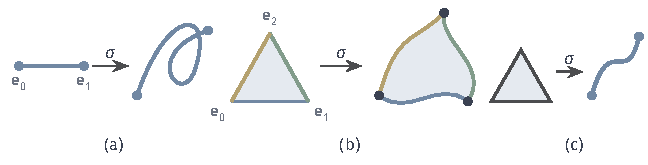
\includegraphics[width=109.657mm]{figures/04-spaces-measures-and-geometry/01-topology-and-metric/tikz/homol-singular-simplices/figure.pdf}
  \caption{奇异单形是连续映射，其像可以弯曲或退化。(a)$\sigma:\Delta^1\to X$是一条路径，允许自相交。(b)$\sigma:\Delta^2\to X$，蓝、绿、黄三条边是三个面$\sigma\circ\delta_2,\sigma\circ\delta_0,\sigma\circ\delta_1$的像。(c)$\Delta^2$可以被整个压到一条曲线上，它仍是一个合法的二维奇异单形。}
  \label{fig:homol-singular-simplices}
\end{BookInlineFigure}

$S_k(X)$通常是无穷维的：$X$中的每个点都是一个$0$维奇异单形，每条路径都是一个$1$维奇异单形，如图~\ref{fig:homol-singular-simplices}所示。但每个奇异链只涉及有限个奇异单形，所以下面的线性代数操作都是有限的。

\paragraph{奇异边界}
在复形中，$k$-单纯形的第$i$个面是去掉第$i$个顶点。对奇异单形，把它限制到$\Delta^k$的第$i$个面上即可。先用下面的映射把低一维的标准单纯形放到这个面上，它在第$i$个位置插入零：
\[
 \delta_i:\Delta^{k-1}\to\Delta^k,\qquad
 \delta_i(t_0,\ldots,t_{k-1})=(t_0,\ldots,t_{i-1},0,t_i,\ldots,t_{k-1}).
\]

这个映射把$\Delta^{k-1}$线性地送到$\Delta^k$中与$\bm e_i$相对的面上，并保持其余顶点的次序。奇异单形的边界就定义为
\begin{equation}
 \partial_k\sigma=\sum_{i=0}^k(-1)^i\,\sigma\circ\delta_i,
 \label{eq:homol-singular-boundary}
\end{equation}
线性延拓到$S_k(X)$。每个$\sigma\circ\delta_i$都是连续映射的复合，是$(k-1)$维奇异单形。对路径$\sigma$，
\[
 \partial_1\sigma=\sigma\circ\delta_0-\sigma\circ\delta_1=\sigma(\bm e_1)-\sigma(\bm e_0),
\]
仍是终点减起点。

\begin{example}[平面上一个奇异三角形的边界]
\label{ex:homol-singular-boundary}
取$X=\mathbb R^2$与线性映射
\[
 \sigma(t_0,t_1,t_2)=(t_1,t_2).
\]
它把$\Delta^2$送到顶点为$(0,0),(1,0),(0,1)$的三角形上，$\bm e_0,\bm e_1,\bm e_2$依次对应这三点。三个面依次是
\begin{align*}
 (\sigma\circ\delta_0)(s_0,s_1)&=\sigma(0,s_0,s_1)=(s_0,s_1),\\
 (\sigma\circ\delta_1)(s_0,s_1)&=\sigma(s_0,0,s_1)=(0,s_1),\\
 (\sigma\circ\delta_2)(s_0,s_1)&=\sigma(s_0,s_1,0)=(s_1,0).
\end{align*}
它们分别是从$(1,0)$到$(0,1)$、从$(0,0)$到$(0,1)$、从$(0,0)$到$(1,0)$的线段。由式~\eqref{eq:homol-singular-boundary}，
\[
 \partial_2\sigma=\sigma\circ\delta_0-\sigma\circ\delta_1+\sigma\circ\delta_2,
\]
正负号使三段路径沿三角形绕行一周，与单纯情形的$\partial_2[v_0,v_1,v_2]$一致。
\end{example}

\begin{lemma}[奇异边界的边界为零]
\label{lem:homol-singular-boundary-squared}
对$i<j$，作为$\Delta^{k-2}\to\Delta^k$的映射，
\begin{equation}
 \delta_j\circ\delta_i=\delta_i\circ\delta_{j-1}.
 \label{eq:homol-face-identity}
\end{equation}
因此$\partial_{k-1}\circ\partial_k=0$。
\end{lemma}

\begin{proof}
式~\eqref{eq:homol-face-identity}的两边都在第$i$与第$j$个位置插入零，其余坐标依次排在剩下的位置上。左边先在第$i$位插零，再在第$j$位插零。右边先在第$j-1$位插零，再在更靠前的第$i$位插零，使前一个零后移到第$j$位。所以两边相同。

展开两次边界，得到
\[
 \partial\partial\sigma=\sum_{j=0}^k\sum_{i=0}^{k-1}(-1)^{i+j}\sigma\circ\delta_j\circ\delta_i.
\]
按$i<j$与$i\geq j$分成两组。第一组用式~\eqref{eq:homol-face-identity}改写，再令$j'=j-1\geq i$，得到
\[
 \sum_{i<j}(-1)^{i+j}\sigma\circ\delta_i\circ\delta_{j-1}
 =-\sum_{i\leq j'}(-1)^{i+j'}\sigma\circ\delta_i\circ\delta_{j'}.
\]
第二组把求和字母改写为$a=j\leq b=i$，得到
\[
 \sum_{a\leq b}(-1)^{a+b}\sigma\circ\delta_a\circ\delta_b.
\]
两组逐项相消。
\end{proof}

这与定理~\ref{thm:homol-boundary-squared}是同一个机制：去掉两个顶点的两种先后次序以相反的符号出现。于是$(S_k(X),\partial_k)$是链复形。

\begin{definition}[奇异同调]
\label{def:homol-singular-homology}
拓扑空间$X$的$k$维（实系数）\term{奇异同调}（singular homology）空间定义为
\begin{equation}
 H_k(X)=\ker\partial_k/\operatorname{im}\partial_{k+1}.
 \label{eq:homol-singular-homology}
\end{equation}
闭链、边界链与同调类的说法与单纯情形相同。
\end{definition}

\begin{BookInlineTable}
  \centering
  \caption{单纯同调与奇异同调}
  \label{tab:homol-simplicial-vs-singular}
  \begin{tabular}{lll}
    \toprule
    & 单纯同调 & 奇异同调 \\
    \midrule
    输入 & 有限复形 & 任意拓扑空间 \\
    $k$维基向量 & $k$-单纯形，有限个 & 连续映射$\Delta^k\to X$ \\
    取边界 & 去掉第$i$个顶点 & 限制到第$i$个面 \\
    可否直接求秩 & 可以 & 不可以，维数无穷 \\
    是否依赖选择 & 依赖复形 & 只依赖空间 \\
    \bottomrule
  \end{tabular}
\end{BookInlineTable}

表~\ref{tab:homol-simplicial-vs-singular}比较了两种构造。奇异同调的优点和缺点恰好与单纯同调互补，第~\ref{sec:homol-simplicial-singular}小节要把二者接起来。

\paragraph{零维同调与路径分支}
零维奇异单形就是$X$中的点，一维奇异单形就是路径，其边界是终点减起点。所以零维同调的计算与定理~\ref{thm:homol-h0-components}平行，只是图的路径换成了空间中的路径。

\begin{theorem}[零维奇异同调计数路径分支]
\label{thm:homol-singular-h0}
设$X$的路径分支为$\{P_\alpha\}$，从每个$P_\alpha$中取一点$x_\alpha$。则$\{[x_\alpha]\}$是$H_0(X)$的一组基；特别地，$X$非空且路径连通时，$H_0(X)\cong\mathbb R$。
\end{theorem}

\begin{proof}
若$x,y$在同一路径分支中，取从$y$到$x$的路径$\sigma$，则$x-y=\partial_1\sigma$，二者同调。所以$\{[x_\alpha]\}$张成$H_0(X)$。

对每个分支$P_\alpha$定义线性函数$\varphi_\alpha$：把$0$维链在$P_\alpha$中各点上的系数相加。路径$\sigma$的像是路径连通集，起点与终点同属一个路径分支，所以$\varphi_\alpha(\partial_1\sigma)=0$，$\varphi_\alpha$在边界链上为零，在$H_0(X)$上有定义。

若有限组合$\sum\lambda_\alpha[x_\alpha]=0$，用$\varphi_\beta$作用得$\lambda_\beta=0$，所以它们线性无关。
\end{proof}

\paragraph{连续映射诱导的同调映射}
奇异同调的好处在于，任何连续映射都能直接作用在链上：奇异单形与连续映射复合，仍是奇异单形。单纯同调做不到这一点，一个连续映射通常不把单纯形送到单纯形。

\begin{theorem}[连续映射诱导同调映射]
\label{thm:homol-induced-map}
设$f:X\to Y$连续。令$f_\#\sigma=f\circ\sigma$并线性延拓，则$f_\#:S_k(X)\to S_k(Y)$是链映射，诱导线性映射$f_*:H_k(X)\to H_k(Y)$。并且$(\operatorname{id}_X)_*=\operatorname{id}$；若$g:Y\to Z$连续，则
\begin{equation}
 (g\circ f)_*=g_*\circ f_*.
 \label{eq:homol-functoriality}
\end{equation}
\end{theorem}

\begin{proof}
连续映射的复合满足结合律，所以
\[
 f\circ(\sigma\circ\delta_i)=(f\circ\sigma)\circ\delta_i.
\]
对式~\eqref{eq:homol-singular-boundary}逐项作用，得到
\[
 \partial f_\#\sigma=f_\#\partial\sigma,
\]
所以$f_\#$是链映射，由引理~\ref{lem:homol-chain-map-induces}诱导$f_*$。

在链层面，$(\operatorname{id}_X)_\#$是恒等映射，并且
\[
 (g\circ f)_\#\sigma=g\circ f\circ\sigma=g_\#f_\#\sigma,
\]
下降到同调即得后两条。
\end{proof}

若$f$是同胚，$f^{-1}$也连续，由式~\eqref{eq:homol-functoriality}，
\[
 f_*\circ(f^{-1})_*=(\operatorname{id}_Y)_*=\operatorname{id},
\]
另一侧同理，所以$f_*$是同构。同胚的空间有同构的奇异同调，Betti数是\term{拓扑不变量}（topological invariant）。反过来说，只要Betti数不同，两个空间就不同胚。

\subsection{单纯同调与奇异同调}
\label{sec:homol-simplicial-singular}

奇异同调对一切空间有定义，但$S_k(X)$是无穷维的，无法直接求秩。单纯同调能用有限矩阵计算，却依赖三角剖分。要把两者的长处结合起来，需要在有限复形上比较这两种链。

\paragraph{比较映射}
设$\mathcal K$是有限单纯复形，$V$上取定全序。一个单纯形可以直接看成一个奇异单形：把标准单纯形线性地放到它上面。对每个按递增次序排列的$k$-单纯形$[v_0,\ldots,v_k]$，令
\begin{equation}
 \theta[v_0,\ldots,v_k]:\Delta^k\to\lvert\mathcal K\rvert,\qquad(t_0,\ldots,t_k)\mapsto\sum_{i=0}^kt_i\bm e_{v_i},
 \label{eq:homol-comparison}
\end{equation}
这里$\bm e_{v_i}$是式~\eqref{eq:homol-realization}中顶点$v_i$对应的基向量。线性延拓，就得到链空间之间的映射
\[
 \theta:C_k(\mathcal K)\to S_k(\lvert\mathcal K\rvert).
\]

$\theta$只对递增排列的基向量定义。其他排列给出的奇异单形是同一个映射与坐标置换的复合，在$S_k$中是另一个基向量，并不等于它的$\pm1$倍；所以这里只能先固定定向，再线性延拓。

$\theta$是链映射。$\theta[v_0,\ldots,v_k]\circ\delta_i$在第$i$个坐标为零的点上取值，恰为$\theta[v_0,\ldots,\widehat{v_i},\ldots,v_k]$，而后者仍按递增次序排列。对式~\eqref{eq:homol-singular-boundary}与式~\eqref{eq:homol-boundary}逐项比较，符号$(-1)^i$也相同。所以$\partial\theta=\theta\partial$，由引理~\ref{lem:homol-chain-map-induces}，$\theta$诱导同调之间的线性映射$\theta_*$。

\begin{theorem}[单纯同调与奇异同调同构]
\label{thm:homol-simplicial-singular}
对有限单纯复形$\mathcal K$与一切$k$，
\begin{equation}
 \theta_*:H_k(\mathcal K)\to H_k(\lvert\mathcal K\rvert)
 \label{eq:homol-simplicial-singular}
\end{equation}
是同构。
\end{theorem}

这个定理的证明需要用到相对同调的长正合列、奇异链的重心细分（切除定理）与五引理，篇幅较长，读者可查阅代数拓扑教材中单纯同调与奇异同调等价的论证。这里说明它的含义与机制。

设想把复形一块一块搭起来，每次加入一个$k$-单纯形，它的边界已经在原来的复形里。这一步在两种同调上引起的变化相同：它只影响$k$维与$k-1$维，要么填掉一个$(k-1)$维的类，要么产生一个新的$k$维类，这由新单纯形的边界在旧复形中是否已是边界决定。证明的技术部分是说明奇异同调确实只“看到”这一块单纯形的相对信息，重心细分正是用来把任意奇异单形切小，切到每一小块都落在某个单纯形的邻域内。

逐块比较的结果是$\theta_*$在每一步都保持同构，从空复形出发归纳，就得到全部同构。

\paragraph{零维情形的核对}
在零维，定理~\ref{thm:homol-simplicial-singular}可以直接验证。由引理~\ref{lem:homol-simplices-intersect}，$\lvert\mathcal K\rvert$中每个点属于它的支撑所对应的凸包，凸包中的线段把它连到一个顶点；每条边的实现是连接两个端点的线段。所以一维骨架同一分量中的顶点在$\lvert\mathcal K\rvert$中属于同一路径分支，每个路径分支都含有顶点。

反过来，设$C$是一维骨架的一个分量，$\mathcal K_C$是顶点都在$C$中的单纯形组成的子复形。每个单纯形的顶点两两相邻，因而同属一个分量，所以$\lvert\mathcal K\rvert$是各个$\lvert\mathcal K_C\rvert$的不交并。

每个$\lvert\mathcal K_C\rvert$是有限个闭凸包之并，是闭集；它的补集是其余有限个闭集之并，也是闭集。这些闭集两两不交、并为整个空间，而一条路径的像是连通集，所以它只能落在其中一个之内。不同分量的顶点因而不在同一路径分支中。

于是两种零维同调都以“每个分量取一个顶点”为基，$\theta_*$把$[u_j]$送到$[u_j]$，是同构。

\paragraph{用三角剖分计算连续空间的同调}
定理~\ref{thm:homol-simplicial-singular}与同调的拓扑不变性合起来，给出计算连续空间同调的方法：找一个三角剖分$X\cong\lvert\mathcal K\rvert$，再按第~\ref{sec:homol-homology-spaces}小节求边界矩阵的秩。奇异同调不依赖任何选择，所以同一个空间的不同三角剖分必然给出同构的单纯同调。

\begin{example}[圆周、圆盘与球面的同调]
\label{ex:homol-sphere-homology}
由例~\ref{ex:homol-triangle-circle}，$S^1\cong\lvert\mathcal T_1\rvert$，$D^2\cong\lvert\mathcal T_2\rvert$，$S^2\cong\lvert\mathcal S\rvert$。由例~\ref{ex:homol-triangle-homology}与例~\ref{ex:homol-tetrahedron-homology}，
\[
 \begin{aligned}
 S^1&:\ \beta_0=\beta_1=1,\\
 D^2&:\ \beta_0=1,\\
 S^2&:\ \beta_0=1,\ \beta_1=0,\ \beta_2=1,
 \end{aligned}
\]
其余Betti数全为零。特别地，$S^1$与$S^2$不同胚，$S^1$与$D^2$也不同胚。
\end{example}

这些结论单从奇异同调的定义很难得到。例如$S^1$上有无穷多个从$\Delta^2$出发的连续映射，直接证明$H_2(S^1)=0$需要排除所有可能的奇异闭链。定理~\ref{thm:homol-simplicial-singular}把这一问题转化为三条边和三个顶点的矩阵计算。

\subsection{同伦不变性}
\label{sec:homol-homotopy-invariance}

第~\ref{sec:homol-homotopy}节说环带与圆周“有同样的洞”，却只能凭直观。现在可以证明：同伦的映射诱导相同的同调映射，因而同伦等价的空间有同构的同调。

\paragraph{棱柱构造}
设$H:X\times[0,1]\to Y$是从$f$到$g$的同伦。对$X$中的一条闭链$\bm z$，$H$把$\bm z\times[0,1]$扫成一块“柱面”，柱面的底是$f_\#\bm z$，顶是$g_\#\bm z$，见图~\ref{fig:homol-prism}(c)。若$\bm z$有边界，边界扫出侧面；$\bm z$闭合时没有侧面，于是$g_\#\bm z-f_\#\bm z$恰好是柱面的边界。

\begin{BookInlineFigure}
  \centering
  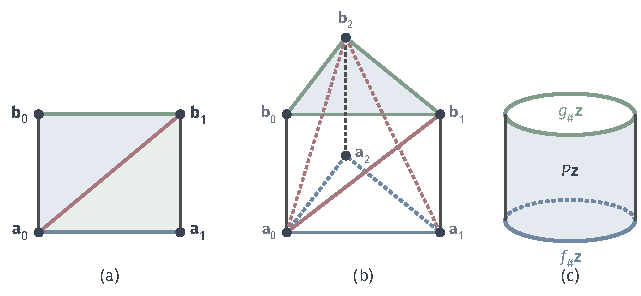
\includegraphics[width=108.511mm]{figures/04-spaces-measures-and-geometry/01-topology-and-metric/tikz/homol-prism/figure.pdf}
  \caption{棱柱的切分与同伦扫出的柱面。(a)$\Delta^1\times[0,1]$被红色对角线切成两个三角形，底边对应$f\circ\sigma$，顶边对应$g\circ\sigma$。(b)$\Delta^2\times[0,1]$被红色线段切成三个四面体$[\bm a_0,\bm b_0,\bm b_1,\bm b_2]$、$[\bm a_0,\bm a_1,\bm b_1,\bm b_2]$、$[\bm a_0,\bm a_1,\bm a_2,\bm b_2]$。(c)闭链$\bm z$被同伦扫成柱面，柱面的边界是顶$g_\#\bm z$减底$f_\#\bm z$。}
  \label{fig:homol-prism}
\end{BookInlineFigure}

要把这个柱面写成奇异链，需要把棱柱$\Delta^k\times[0,1]$切成若干个$(k+1)$维单纯形。记棱柱的底面顶点为$\bm a_i=(\bm e_i,0)$，顶面顶点为$\bm b_i=(\bm e_i,1)$，其中$i=0,\ldots,k$。

对棱柱中的点$\bm u_0,\ldots,\bm u_{k+1}$，记
\[
 \langle\bm u_0,\ldots,\bm u_{k+1}\rangle:\Delta^{k+1}\to\Delta^k\times[0,1]
\]
为把$\bm e_m$送到$\bm u_m$的线性映射，棱柱是凸集，所以它的像在棱柱中。对$X$中的奇异单形$\sigma$，令
\[
 F_\sigma=H\circ(\sigma\times\operatorname{id}_{[0,1]}):\Delta^k\times[0,1]\to Y,
\]
定义\term{棱柱算子}（prism operator）
\begin{equation}
 P\sigma=\sum_{i=0}^k(-1)^i\,F_\sigma\circ\langle\bm a_0,\ldots,\bm a_i,\bm b_i,\ldots,\bm b_k\rangle,
 \label{eq:homol-prism}
\end{equation}
它属于$S_{k+1}(Y)$，并线性延拓为$P:S_k(X)\to S_{k+1}(Y)$。

式中第$i$个单纯形从底面的前$i+1$个顶点出发，在第$i$个顶点处“爬上”顶面，再走完顶面的其余顶点。这$k+1$个单纯形拼成整个棱柱；下面的证明只用到它们的边界之间的相消关系。

\begin{example}[低维的棱柱]
\label{ex:homol-prism-low}
$k=0$时，$\sigma$是一点$x$，$P\sigma$是路径$t\mapsto H(x,t)$，边界为
\[
 \partial P\sigma=g(x)-f(x).
\]

$k=1$时，$\sigma$是路径，正方形$\Delta^1\times[0,1]$被对角线切成两个三角形：
\[
 P\sigma=F_\sigma\circ\langle\bm a_0,\bm b_0,\bm b_1\rangle-F_\sigma\circ\langle\bm a_0,\bm a_1,\bm b_1\rangle.
\]

省略复合号，按式~\eqref{eq:homol-singular-boundary}分别展开两项：
\begin{align*}
 \partial\bigl(F_\sigma\langle\bm a_0,\bm b_0,\bm b_1\rangle\bigr)&=F_\sigma\langle\bm b_0,\bm b_1\rangle-F_\sigma\langle\bm a_0,\bm b_1\rangle+F_\sigma\langle\bm a_0,\bm b_0\rangle,\\
 \partial\bigl(F_\sigma\langle\bm a_0,\bm a_1,\bm b_1\rangle\bigr)&=F_\sigma\langle\bm a_1,\bm b_1\rangle-F_\sigma\langle\bm a_0,\bm b_1\rangle+F_\sigma\langle\bm a_0,\bm a_1\rangle.
\end{align*}

两式相减，对角线$\langle\bm a_0,\bm b_1\rangle$相消，剩下
\[
 \partial P\sigma=F_\sigma\langle\bm b_0,\bm b_1\rangle+F_\sigma\langle\bm a_0,\bm b_0\rangle-F_\sigma\langle\bm a_1,\bm b_1\rangle-F_\sigma\langle\bm a_0,\bm a_1\rangle.
\]

四项依次是$g\circ\sigma$、起点的轨迹、终点的轨迹与$f\circ\sigma$。由于$\partial\sigma=\sigma(\bm e_1)-\sigma(\bm e_0)$，这正是
\[
 \partial P\sigma=g_\#\sigma-f_\#\sigma-P\partial\sigma,
\]
正方形的边界等于顶减底，再减去两条侧边。
\end{example}

例~\ref{ex:homol-prism-low}中的恒等式对一般的$k$也成立，图~\ref{fig:homol-prism}(a)(b)画出了$k=1,2$的切分。

\begin{lemma}[棱柱恒等式]
\label{lem:homol-prism-identity}
对一切$k\geq0$与$\sigma\in S_k(X)$，
\begin{equation}
 \partial P\sigma+P\partial\sigma=g_\#\sigma-f_\#\sigma.
 \label{eq:homol-prism-identity}
\end{equation}
\end{lemma}

\begin{proof}
记$[\cdots]$为$F_\sigma\circ\langle\cdots\rangle$，只需对奇异单形$\sigma$验证。对式~\eqref{eq:homol-prism}的第$i$项取边界，去掉第$j$个顶点：$j\leq i$时去掉的是$\bm a_j$，符号为$(-1)^j$；$j\geq i$时去掉的是$\bm b_j$，它位于第$j+1$个位置，符号为$(-1)^{j+1}$。于是$\partial P\sigma$是下面两组之和：
\begin{gather*}
 \sum_{j\leq i}(-1)^{i+j}[\bm a_0,\ldots,\widehat{\bm a_j},\ldots,\bm a_i,\bm b_i,\ldots,\bm b_k],\\
 \sum_{j\geq i}(-1)^{i+j+1}[\bm a_0,\ldots,\bm a_i,\bm b_i,\ldots,\widehat{\bm b_j},\ldots,\bm b_k].
\end{gather*}

先看$i=j$的项。第一组中$i=j$的项是$[\bm a_0,\ldots,\bm a_{i-1},\bm b_i,\ldots,\bm b_k]$，第二组中下标为$i-1$、去掉$\bm b_{i-1}$的项是它的相反数，因为符号为$(-1)^{2i-1}$。对$i=1,\ldots,k$，二者相消。剩下第一组$i=j=0$与第二组$i=j=k$的项：
\[
 [\bm b_0,\ldots,\bm b_k]=g\circ\sigma,\qquad-[\bm a_0,\ldots,\bm a_k]=-f\circ\sigma.
\]

再看$i\neq j$的项。去掉$\bm a_j$（$j<i$）或$\bm b_j$（$j>i$）后，剩下的单纯形恰好是第$j$个面$\sigma\circ\delta_j$所对应棱柱中的一块：前者是第$i-1$块，后者是第$i$块。这是因为$\delta_j\times\operatorname{id}$把较小棱柱的顶点按次序线性地送到这些顶点上，并满足
\[
 F_\sigma\circ(\delta_j\times\operatorname{id})=F_{\sigma\circ\delta_j}.
\]

按定义展开
\[
 P\partial\sigma=\sum_j(-1)^jP(\sigma\circ\delta_j)
 =\sum_{i>j}(-1)^{i+j-1}[\cdots\widehat{\bm a_j}\cdots]+\sum_{i<j}(-1)^{i+j}[\cdots\widehat{\bm b_j}\cdots],
\]
它恰好是$\partial P\sigma$中$i\neq j$各项的相反数。三部分相加，即得式~\eqref{eq:homol-prism-identity}。
\end{proof}

式~\eqref{eq:homol-prism-identity}的几何含义是：柱面的边界等于顶减底，再减去边界扫出的侧面。这是例~\ref{ex:homol-prism-low}中“正方形的边界”在一般维数上的写法。

\begin{theorem}[同伦不变性]
\label{thm:homol-homotopy-invariance}
若连续映射$f,g:X\to Y$同伦，则
\begin{equation}
 f_*=g_*:H_k(X)\to H_k(Y)
 \label{eq:homol-homotopy-invariance}
\end{equation}
对一切$k$成立。因此，若$f:X\to Y$是同伦等价，则$f_*$是同构；同伦等价的空间有同构的奇异同调。
\end{theorem}

\begin{proof}
对闭链$\bm z$，由引理~\ref{lem:homol-prism-identity}，
\[
 g_\#\bm z-f_\#\bm z=\partial P\bm z+P\partial\bm z=\partial P\bm z,
\]
右端是边界链，所以$g_*[\bm z]=f_*[\bm z]$。

若$h$是$f$的同伦逆，由定理~\ref{thm:homol-induced-map}与刚才的结论，
\[
 h_*f_*=(h\circ f)_*=(\operatorname{id}_X)_*=\operatorname{id},
\]
同理$f_*h_*=\operatorname{id}$，所以$f_*$是同构。
\end{proof}

这个结论称为同调的\term{同伦不变性}（homotopy invariance）。它在第~\ref{sec:homol-homotopy}节与本节之间架起桥梁：同伦等价保留的代数信息，至少包括全部Betti数。

\paragraph{单点与可缩空间}
单点空间$\{p\}$在每个维数恰有一个奇异单形$\sigma_k$（常值映射），并且$\sigma_k\circ\delta_i=\sigma_{k-1}$。由式~\eqref{eq:homol-singular-boundary}，
\[
 \partial_k\sigma_k=\sum_{i=0}^k(-1)^i\sigma_{k-1}=
 \begin{cases}0,&k\text{为奇数},\\ \sigma_{k-1},&k\geq2\text{为偶数}.\end{cases}
\]

所以$\partial_1=0$，$\partial_2$是同构，$\partial_3=0$，$\partial_4$是同构，依此类推。$k$为奇数时$\ker\partial_k=S_k$被$\operatorname{im}\partial_{k+1}$占满；$k\geq2$为偶数时$\ker\partial_k=0$。于是
\[
 H_0(\{p\})\cong\mathbb R,\qquad H_k(\{p\})=0\ (k\geq1).
\]
由定理~\ref{thm:homol-homotopy-invariance}，可缩空间（如区间、圆盘、$\mathbb R^n$）的同调与单点相同。

\paragraph{环带与圆周}
回到本章开头的问题。由例~\ref{ex:homol-annulus-retraction}与定理~\ref{thm:homol-retract-equivalence}，包含映射$i:S^1\to A$是同伦等价。由定理~\ref{thm:homol-homotopy-invariance}，$i_*$是同构，所以
\[
 H_1(A)\cong H_1(S^1)\cong\mathbb R.
\]
更具体地，环绕圆周一周的一维闭链，在环带中仍是不能填掉的闭链；环带比圆周多出的“厚度”被形变收缩压平，不产生新的同调类。

由此兑现第~\ref{sec:homol-homotopy-equivalence}小节的承诺：$H_1(A)\neq0=H_1(\{p\})$，所以环带不可缩。

同一论证还说明圆盘不能回缩到边界圆周上。若$r:D^2\to S^1$是回缩，$j:S^1\to D^2$为包含，则$r\circ j=\operatorname{id}_{S^1}$，于是$r_*\circ j_*$是$H_1(S^1)\cong\mathbb R$上的恒等映射。可是$j_*$经过$H_1(D^2)=0$，复合只能为零，矛盾。

\paragraph{同调不能判定什么}
同伦不变性同时划出了同调的边界。圆盘与单点同伦等价，同调相同，却不同胚；所以同调相同不能推出同胚，这一点在第~\ref{sec:homol-homology-spaces}小节已经用复形看到。

同调相同也不能推出同伦等价。环面与“两个圆周和一个球面粘在一点”的空间，Betti数都是$(1,2,1)$，却不同伦等价；区分它们要用基本群或同调环等更细的工具，证明需要另外建立这些工具。同调是检验“不同”的工具：Betti数不同，就足以断定两个空间既不同胚，也不同伦等价。

\section{本章小结}
\label{sec:homol-summary}

本章开头问：三角形框与三角形纸片有同样的顶点和边，怎样用代数量区分“有洞”与“被填上”；环带与圆周不同胚，怎样说明它们有同样的洞。前一个问题由单纯同调回答，后一个问题由同伦与同伦不变性回答。

同伦用乘积空间$X\times[0,1]$上的连续映射描述映射的连续变形，它是与复合相容的等价关系。把“互逆”放宽为“复合同伦于恒等映射”，得到同伦等价；与单点同伦等价的空间称为可缩空间，凸集都可缩。形变收缩把空间收回子空间并在过程中固定子空间，包含映射因而是同伦等价，环带由此与圆周同伦等价。同伦等价比同胚宽松：区间、圆盘和单点同伦等价，却两两不同胚。只有回缩而没有形变则不够，两点离散空间就是例子。

有限单纯复形用对取面封闭的顶点子集族记录点、边和各维填充，一维复形就是图。几何实现把每个单纯形换成标准单纯形，沿公共面粘合；它既是商空间，又同胚于欧氏空间中以标准基向量为顶点的凸包之并，其中两个单纯形只在公共面上相交。画在纸上的交叉不是复形中的点。

单纯同调在实数系数下取链空间$C_k(\mathcal K)\cong\mathbb R^{n_k}$，由交错取面定义边界映射，并验证$\partial\circ\partial=0$。闭链是边界映射的核，边界链是高一维边界映射的像，同调是二者之商，Betti数为$\beta_k=n_k-\operatorname{rank}\bm D_k-\operatorname{rank}\bm D_{k+1}$。$\beta_0$计数一维骨架的连通分量；三角形边界的$\beta_1=1$，填实后变为$0$；四面体表面的$\beta_2=1$。Euler示性数等于Betti数的交错和，可以核对手算。链映射诱导同调映射；比较子复形与大复形时，诱导映射能指出哪个环被填掉，单看Betti数做不到。

奇异同调以标准单纯形到空间的连续映射为基，对一切拓扑空间有定义，零维同调计数路径分支，连续映射诱导同调映射，同胚给出同构。在有限复形上，把单纯形看作线性的奇异单形，得到的比较映射在同调上是同构，本章只证明了零维情形并解释了一般机制；它使连续空间的同调可以用三角剖分的边界矩阵计算，并与三角剖分的选择无关。棱柱构造证明同伦映射诱导相同的同调映射，所以同伦等价的空间有同构的同调。由此，环带与圆周的$\beta_1$都是$1$，环带不可缩，圆盘不能回缩到边界圆周。

同调的使用有明确的方向：Betti数不同，就足以断定两个空间既不同胚，也不同伦等价；Betti数相同则什么也不能断定，圆盘与单点就是同调相同而不同胚的例子。流形上的同调在第~\ref{chap:manifold-basics}章起继续使用，从有限点云恢复同调、沿一列复形追踪诱导映射的持久同调在第~\ref{chap:manifold-recovery}章展开。下一部分转向另一类问题：不再研究连续变形与孔洞，而是在第~\ref{chap:measure}章度量集合的大小。

